\documentclass{article}

\usepackage[utf8]{inputenc}
\usepackage{longtable}
\usepackage{authblk}
\usepackage{adjustbox}
\usepackage{natbib}

%Creación de títulos del artículo
\title{Índices de Desarrollo Humano de Colombia}

\author[1]{\normalsize Andrés Esteban Acero}
\affil[1]{\small  Doctorado en Ingeniería Industrial, Facultad de Ingeniería,Universidad de los Andes\\
\texttt{{ae.acero539@uniandes.edu.co}}}


\date{29 de Junio de 2018}



\usepackage{Sweave}
\begin{document}
\Sconcordance{concordance:Articulo1.tex:Articulo1.Rnw:%
1 20 1 1 0 11 1 1 16 8 1 1 5 1 2 5 1 1 10 1 2 5 1 1 20 1 2 6 1 1 6 12 0 %
1 2 1 1 1 9 13 0 1 2 2 1 2 2 9 1 1 5 1 1 1 4 31 0 1 2 8 1 1 10 1 1 1 12 %
2 1 1 16 1 3 8 1}


\maketitle

\begin{abstract}
El Índice de desarrollo humano es uno de los indicadores compuestos de desarrollo socio-económico máss utilizado en el mundo.Un estudio detallado de los Índices de desarrollo humano en el mundo ha mostrado que esta medida, a pesar de sus detractores, refleja un enfoque integral para el estudio de las condiciones de un país.Además, se mantiene como un reflejo de los esfuerzos de recuperación democrática y humanitaria.  Sin embargo, estudios detallados regionales acerca del uso de este indicador, en especial en países en desarrollo, son pocos y con niveles de análisis inadecuados. Por tanto, este artículo hace un análisis detallado del índice de desarrollo humano para cada uno de los departamentos (estados) de Colombia. Este análisis incluye predicciones acerca de las características demográficas que explican este índice, así como agrupamiento de los niveles de desarrollo regional de acuerdo con este índice. De este estudio se concluye que existen tres niveles diferentes de desarrollo, en los cuales un efecto de centro-periferia es evidente, con zonas de desarrollo menor entre estas dos.
\end{abstract}

\section*{Introducción}
El Índice de desarrollo humano, de acuerdo con \cite{sales_proposal_2018}, fue establecido en 1990 por el programa de Naciones Unidas para el desarrollo como una medida del potencial individual para tener una vida satisfactoria. Esta medida ha sido problematizada por diferentes teóricos del desarrollo por dos aspectos. Primero, establece una diferenciación entre la riqueza de la vida humana sobre la riqueza material o la riqueza económica (\cite{sales_proposal_2018}). Por otro lado, las dificultades estadísticas y la exclusión de los tópicos ambientales han sido problematizados en extensión en los últimos años (\cite{biggeri_towards_2018}). Sin embargo, los beneficios mostrados por el uso de este indicador son y siguen siendo importantes para la investigación en desarrollo. Por tanto, este estudio se centra en el uso del índice de desarrollo humano como una medida de análisis regional.
\clearpage

En el caso del contexto colombiano, vemos que los estudios que buscan entender el índice de desarrollo humano en Colombia son escasos, en especial por falta de datos estadísticos actualizados, entre ellos la no existencia de censos desde hace más de 12 años. Aún con las limitaciones presentadas, el programa de las Naciones Unidas para el desarrollo presentó en el 2011 un informe nacional de desarrollo humano. A partir de esta información, este proyecto de investigación busca la construcción de un marco de análisis estadístico de los resultados de este estudio a nivel regional (para cada uno de los departamentos) que permita concluir acerca de las condiciones actuales de desarrollo de Colombia.


Este documento estárá organizado de la siguiente forma: Primero, en la sección \ref{univariada} en la página \pageref{univariada} se hará un análisis básico de las estadísticas demográficas al igual que el índice de desarrollo. , en la sección \ref{bivariada} en la página \pageref{bivariada} se buscará las relaciones entre las variables bajo estudio. Después, en la sección \ref{regresiones} en la página \pageref{regresiones} se buscará explicar el índice de desarrollo humano en términos de las variables predictoras. Finalmente, se buscarán relaciones espaciales entre las variables que puedan explicar los resultados de este indicador. Para lograr esto, en la sección \ref{espacial} se presentarán los resultados de los conglomerados de acuerdo con el nivel de desarrollo.


\section{Exploración Univariada}\label{univariada}

Esta sección comprende el análisis estadístico de cada una de las variables que van a ser objeto de estudio. Primero, los valores del índice de desarrollo humano (IDH) son analizados. Para este fin, en la página \pageref{barplots} podemos apreciar un histograma de los índices para cada uno de los departamentos de Colombia. En esta gráfica podemos apreciar dos fenómenos interesantes para el estudio. Primero, los niveles máximos y mínimos apreciados en la gráfica con respecto al IDH muestran que, de acuerdo con la distribución por tramos propuesta por Informe de desarrollo humano, los departamento de Colombia se encuentran en rangos medio-medio alto del IDH. Sin embargo, no existe ningún departamento en niveles comparables con los encontrados en países como Estados Unidos o Alemania, pero en niveles similares a los encontrados en la región andina. El segundo aspecto relevante de este resultado es un comportamiento similar a una distribución de probabilidad normal con una pequeña asimetría negativa, lo cual explicaría que tengamos diferencias apreciables (y esperables) en el desarrollo de las regiones.
\clearpage

\begin{figure}[h]
\centering
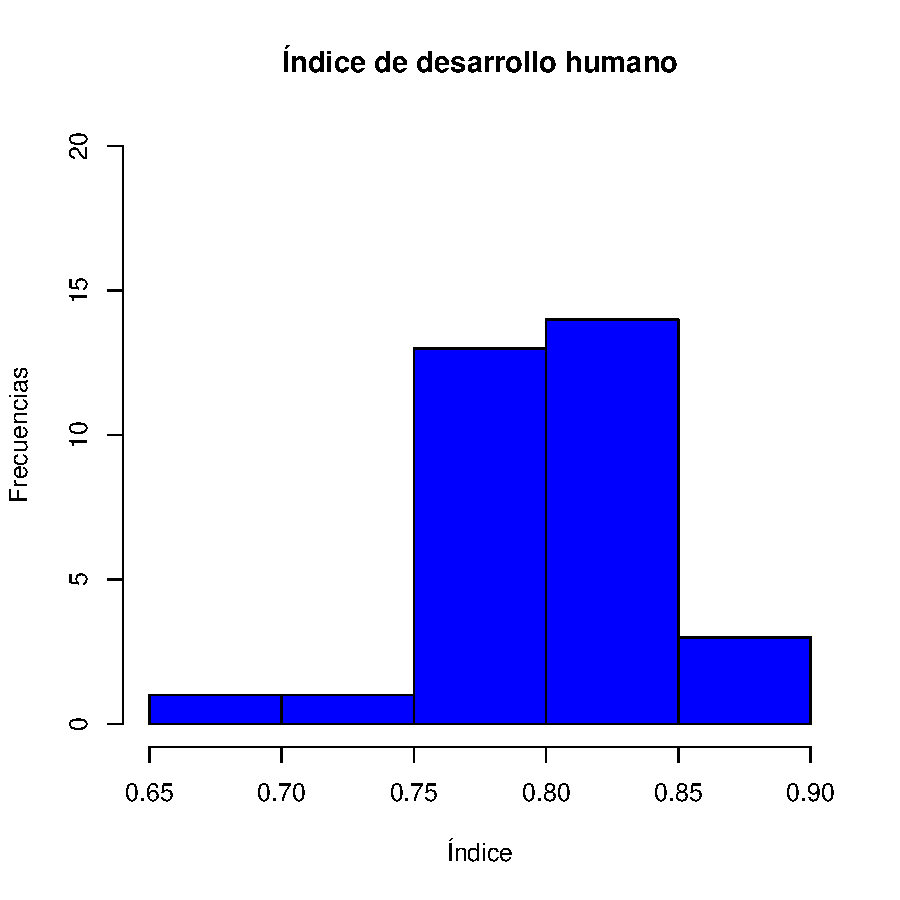
\includegraphics{Articulo1-histIDH}
\caption{Índice de desarrollo humano}
\label{barplots}
\end{figure}

En cuanto a los indicadores demográficos a ser analizados, se escogieron dos altamente relacionados con las diferencias en el desarrollo de las regiones. Así, se escoge la población de cada departamento en las cabeceras de cada uno de los municipios, así como la población fuera de las cabeceras o población rural. Los resultados de estos resultados se muestran en la página \pageref{barplot2}. Un análisis visual de estas gráficas nos permite ver dos aspectos importantes de la demografía colombiana. Primero, cada una de estas gráficas tiene un comportamiento similar a una distribución logística con colas de alto peso (y, en consecuencia, bajos niveles de curtosis). Esto muestra que, al igual con la teoría de redes sociales, podamos encontrar leyes de potencia al analizar la población colombiana. El segundo aspecto relevante de estos resultados es que en Colombia la mayor concentración poblacional se centra en las cabeceras municipales. Esto tiene muchos factores que podrían tener impacto en el IDH, entre los que se encuentran la migración interna, el acceso a recursos o las oportunidades de movilidad laboral o social.
\clearpage

\begin{figure}[h]
\centering
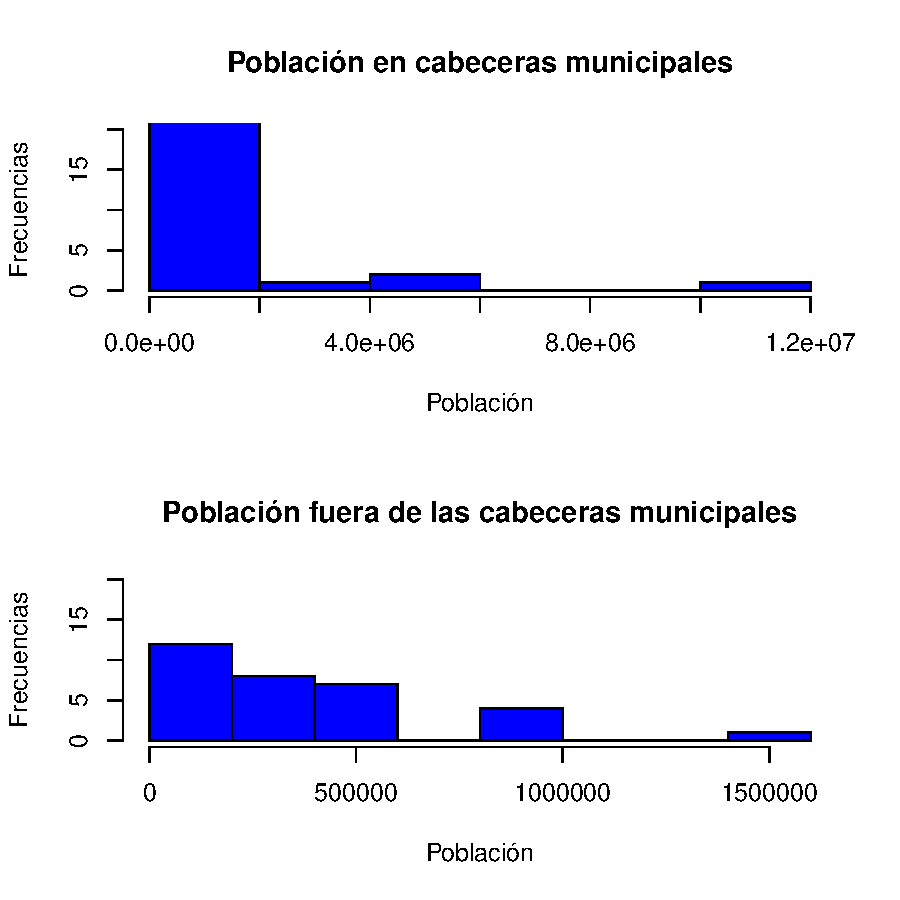
\includegraphics{Articulo1-histPOB}
\caption{Estadísticas demográficas}
\label{barplot2}
\end{figure}

Sin embargo, como se pudo apreciar en la gráfica \ref{barplot2}, la distribución específica de los resultados de la población puede hacer que se presenten problemas tales como descentramiento de los resultados o mayores niveles de dispersión en los datos que hagan imposible llevar a cabo análisis sobre el IDH. En consecuencia, se realizó una transformación en los datos. Para esto, se aplicación una transformación logística a los datos para hacerlos comparables. Los resultados de este proceso en los datos se presentan en la gráfica \ref{barplot3} en la página \pageref{barplot3}.
\clearpage


\begin{figure}[h]
\centering
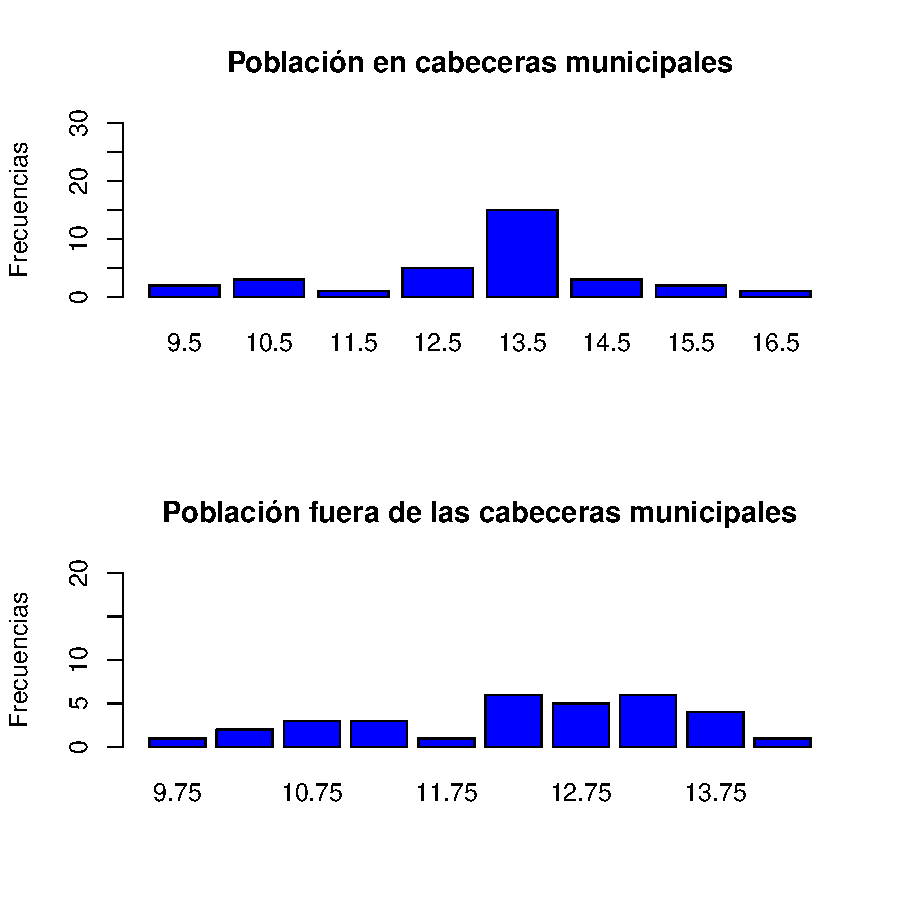
\includegraphics{Articulo1-histNOR}
\caption{Estadísticas demográficas normalizadas}
\label{barplot3}
\end{figure}

En esta sección hemos explorado el comportamiento de las variables de estudio. En la próxima sección de \emph{Exploración Bivariada} estudiaremos el comportamiento de las variables como un conjunto.

\section{Exploración Bivariada}\label{bivariada}
El objetivo de este artículo de investigación reside en el poder explicativo de las variables demográficas a nivel regional en el IDH . Por tanto, es de interés entender la relación de las variables predictoras con respecto al índice de desarrollo humano. Los resultados son presentados en la tabla \ref{corrDem} de la página \pageref{corrDem}.

% Table created by stargazer v.5.2.2 by Marek Hlavac, Harvard University. E-mail: hlavac at fas.harvard.edu
% Date and time: sáb., jul. 07, 2018 - 5:17:52 p. m.
\begin{table}[!htbp] \centering 
  \caption{Correlación del índice de desarrollo humano con las demás variables} 
  \label{corrDem} 
\begin{tabular}{@{\extracolsep{5pt}} cc} 
\\[-1.8ex]\hline 
\hline \\[-1.8ex] 
cabeLog & restoLog \\ 
\hline \\[-1.8ex] 
$0.487$ & $0.177$ \\ 
\hline \\[-1.8ex] 
\end{tabular} 
\end{table} \clearpage

De acuerdo con los resultados presentados en la tabla anterior, vemos que estas variables tienes niveles bajos de correlación con el IDH. Aunque en un estudio estadístico es deseable que la correlación de las variables predictoras con la variable dependiente, en este caso vemos que el mayor nivel de correlación entre la población en zonas urbanas que en zonas rurales. Dado que estas variables se encuentran normalizadas, este efecto no se puede atribuir a una mayor concentración de población. Por el contrario, esto se puede ver como un reflejo de las diferencias en términos de desarrollo entre estas dos poblaciones.

Además, por fines estadísticos, es importante analizar la relación de estas variables entre sí. Los resultados de este análisis podrían dar indicios de problemas en un futuro modelo de regresión, tales como multicolinealidad. Los resultados de las correlaciones entre las variable se presenta en la tabla \ref {corrTbaleX} en la página \pageref{corrTableX}. Además, para entender visualmente si existen problemas en las variables predictoras, se muestra un correlograma en la figura \ref{corrPlotX} en la página \pageref{corrPlotX}.

% Table created by stargazer v.5.2.2 by Marek Hlavac, Harvard University. E-mail: hlavac at fas.harvard.edu
% Date and time: sáb., jul. 07, 2018 - 5:17:58 p. m.
\begin{table}[!htbp] \centering 
  \caption{Correlación entre variables independientes} 
  \label{corrTableX} 
\begin{tabular}{@{\extracolsep{5pt}} ccc} 
\\[-1.8ex]\hline 
\hline \\[-1.8ex] 
 & cabeLog & restoLog \\ 
\hline \\[-1.8ex] 
cabeLog & 1 &  \\ 
restoLog & 0.84 & 1 \\ 
\hline \\[-1.8ex] 
\end{tabular} 
\end{table} 
\begin{figure}[h]
\centering
\begin{adjustbox}{width=7cm,height=7cm,clip}
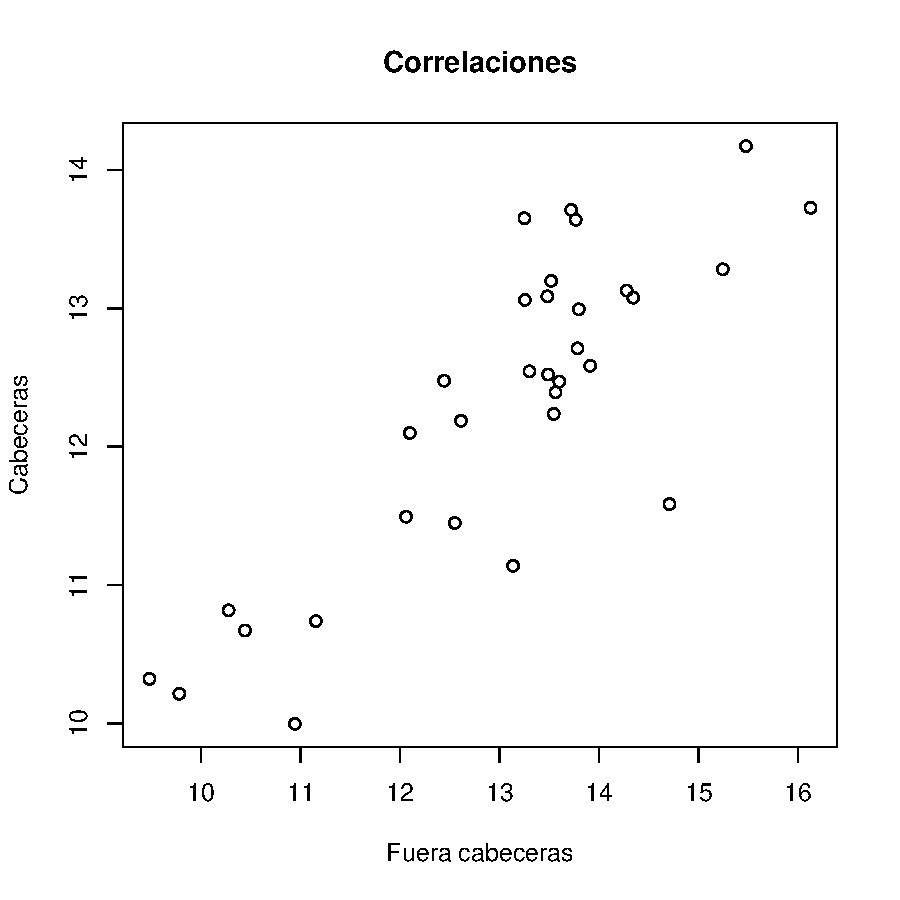
\includegraphics{Articulo1-corrPlotX}
\end {adjustbox}
\caption{correlación entre predictores}
\label{corrPlotX}
\end{figure}

\clearpage

\section{Modelos de Regresión}\label{regresion}

De acuerdo con los resultados del análisis anterior, vemos que son posibles analizar dos modelos para predecir el IDH. El primero es un modelo que trata de explicar la relación entre la población en cabeceras contra los niveles de desarrollo medidos por IDH. En el segundo modelo se incluye además la población fuera de las cabeceras municipales. Los resultados resumidos de estas regresiones se muestran en la Tabla \ref{regresiones} de la página \pageref{regresiones}.



% Table created by stargazer v.5.2.2 by Marek Hlavac, Harvard University. E-mail: hlavac at fas.harvard.edu
% Date and time: sáb., jul. 07, 2018 - 5:17:58 p. m.
\begin{table}[!htbp] \centering 
  \caption{Modelos de Regresión} 
  \label{regresiones} 
\begin{tabular}{@{\extracolsep{5pt}}lcc} 
\\[-1.8ex]\hline 
\hline \\[-1.8ex] 
 & \multicolumn{2}{c}{\textit{Dependent variable:}} \\ 
\cline{2-3} 
\\[-1.8ex] & \multicolumn{2}{c}{IDH} \\ 
\\[-1.8ex] & (1) & (2)\\ 
\hline \\[-1.8ex] 
 cabeLog & 0.013$^{***}$ & 0.031$^{***}$ \\ 
  & (0.004) & (0.007) \\ 
  & & \\ 
 restoLog &  & $-$0.030$^{***}$ \\ 
  &  & (0.010) \\ 
  & & \\ 
 Constant & 0.634$^{***}$ & 0.766$^{***}$ \\ 
  & (0.055) & (0.065) \\ 
  & & \\ 
\hline \\[-1.8ex] 
Observations & 32 & 32 \\ 
R$^{2}$ & 0.238 & 0.425 \\ 
Adjusted R$^{2}$ & 0.212 & 0.385 \\ 
Residual Std. Error & 0.037 (df = 30) & 0.033 (df = 29) \\ 
F Statistic & 9.347$^{***}$ (df = 1; 30) & 10.706$^{***}$ (df = 2; 29) \\ 
\hline 
\hline \\[-1.8ex] 
\textit{Note:}  & \multicolumn{2}{r}{$^{*}$p$<$0.1; $^{**}$p$<$0.05; $^{***}$p$<$0.01} \\ 
\end{tabular} 
\end{table} 
De acuerdo con los resultados presentados, podemos llegar a dos conclusiones importantes. Primero, en el modelo 1 vemos que a medida que aumenta la población en cabeceras municipales, mayor es el nivel de desarrollo de esta región. Aunque este resultado suena contradictorio, el crecimiento de las zonas urbanas en cada departamento podría ser un motor para el desarrollo. En la segunda regresión, además de reflejar los mismos resultados de la primera regresión, vemos que este fenómeno es más claro. A medida que se genere desplazamiento interno hacia zonas urbanas, o por el contrario un crecimiento menor en las regiones rurales generarían mayores niveles de bienestar y desarrollo para el departamento. Este resultado refleja los mismos efectos estudiados previamente, en los cuales la falta de cobertura en los recursos básicos en ciertas regiones hace que se generen mayores niveles de desigualdad social. Para entender mejor este fenómeno, buscaremos casos puntuales que permitan elicitar este resultado.

\clearpage

\section{Exploración Espacial}\label{espacial}


Como acabamos de ver en la Tabla \ref{regresiones} en la página \pageref{regresiones}, si quisieras sintetizar la multidimensionalidad del índice de desarrollo humano, usar las variables demográficas pueden ser buenos predictores.. 

Así, se propone calcular los conglomerados de departamentos usando toda la información de los tres indicadores. Como nuestras variables son continuas utilizaremos un proceso de conglomeración donde las distancia serán calculadas usando la medida {\bf gower} propuestas en \cite{macqueen_methods_nodate}, y para los enlazamientos usaremos la técnica de {\bf K-means}. Los tres niveles de conglomerados se muestran en la Figura \ref{clustmap}.



\begin{figure}[h]
\centering
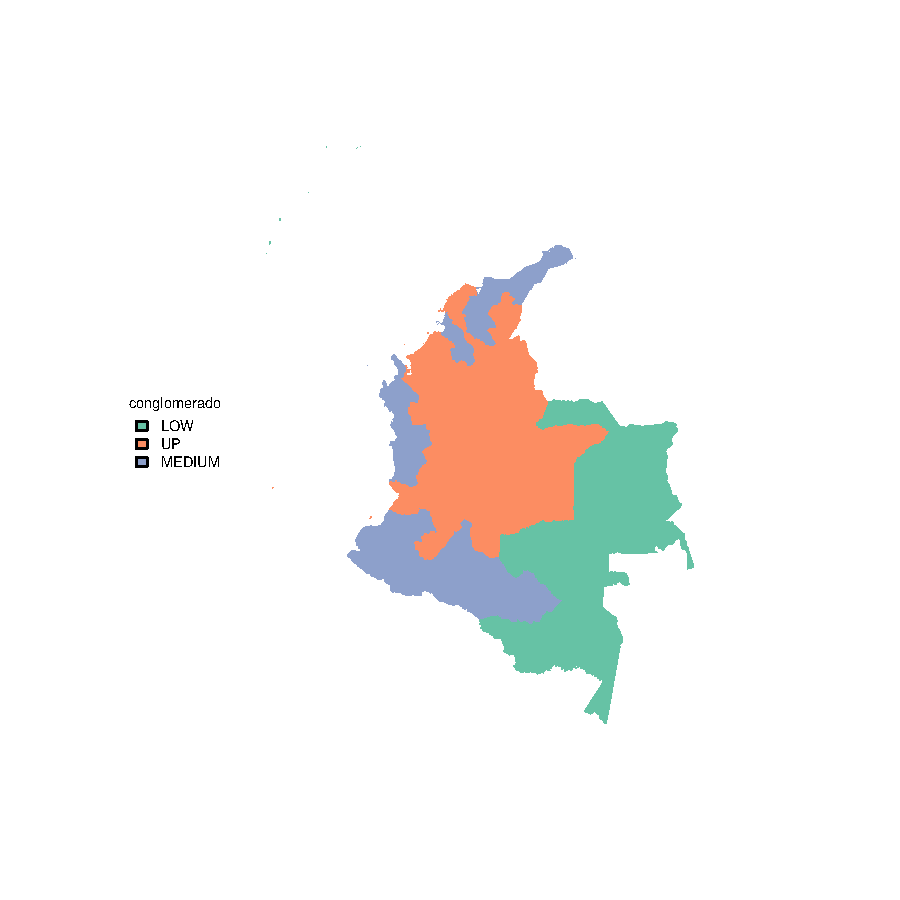
\includegraphics{Articulo1-plotMap1}
\caption{Departamentos conglomerados conglomerados segun sus indicadores sociopolíticos}\label{clustmap}
\end{figure}

Como podemos ver en el mapa, en cada una de las regiones presentadas se presentan diferentes fenómenos, tales como migración forzada en las zonas de alto nivel de desarrollo, mientras que las zonas de bajo nivel de desarrollo hay mayores niveles de acumulación de capital. En futuros análisis sería de interés investigativo el incluir indicadores económicos tales como el producto interno bruto.
\clearpage

\bibliographystyle{apalike}
\renewcommand{\refname}{Bibliografia}
\bibliography{Colombia1}

\end{document}
